\chapter{Evaluation, Results, and Discussion}
\label{ch:results}

\section{Evaluation protocol}
\subsection{Primary and secondary outcomes}
The main question-level comparison uses 924 validation questions and
paper-restricted top-five retrieval. Mean joined retrieval F1 is the
primary outcome; median F1 and mean regret provide complementary
descriptions. All five fixed-size outcomes are available for each
question, making the expected-regret comparison a paired choice among
the same saved actions.

Classification accuracy, macro F1, weighted F1, balanced accuracy,
and top-two accuracy describe the routing targets. Macro F1 gives
each class equal weight, which is useful when the evidence-length
labels are imbalanced. Top-two accuracy is meaningful only when the
model exposes comparable class scores. It is not reported as if
available for unrestricted numeric generation.

The local experiments retain all 924 questions for retrieval, but
their secondary classification diagnostic has a different unit:
2,074 gold-overlapping validation trees from 889 eligible questions.
Those trees are not the same as the 4,620 top-ranked trees used to
construct the primary retrieval outputs. Confusing these denominators
would produce an incorrect interpretation of local classification
accuracy.

\subsection{Paired paper-cluster bootstrap}
The later comparisons use 10,000 bootstrap replicates with seed 42.
Each replicate samples 277 paper identifiers with replacement and
includes all questions belonging to each sampled paper. A paper
sampled twice contributes its questions twice. The replicate statistic
is the question-weighted mean score or paired score difference over
the resulting sample.

For two methods $A$ and $B$, the observed difference is
\begin{equation}
\widehat\Delta_{A-B}=
\frac{1}{N}\sum_{q=1}^{N}
\bigl[\retrievalf^{A}(q)-\retrievalf^{B}(q)\bigr].
\end{equation}
The 2.5th and 97.5th percentiles of the bootstrap differences form
the reported 95\% interval. The same resampled papers are used for
both methods in a pair. This preserves their within-question pairing
and the clustering of questions within papers.

These intervals condition on the saved fitted models and the observed
development sample. They do not include variance from retraining,
hyperparameter search, prompt development, or unobserved datasets.
An interval that includes zero does not prove equivalence, and an
interval that excludes zero does not remove selection bias from
repeated validation use.

\section{Fixed granularity and oracle headroom}
% Generated by scripts/generate_results.py; do not hand-edit.
\begin{table}[htbp]
\centering\small
\caption{Fixed-size top-five retrieval on 924 validation questions.}
\label{tab:fixedresults}
\begin{tabular}{@{}lrrrr@{}}
\toprule
Size / method & Mean F1 & Median F1 & Regret & 95\% interval\\
\midrule
10 & 0.2211 & 0.2074 & 0.1610 & [0.2138, 0.2286]\\
20 & 0.2887 & 0.2809 & 0.0933 & [0.2800, 0.2975]\\
40 & 0.3159 & 0.3092 & 0.0662 & [0.3058, 0.3260]\\
80 & 0.2857 & 0.2666 & 0.0963 & [0.2746, 0.2966]\\
160 & 0.2168 & 0.1838 & 0.1653 & [0.2063, 0.2271]\\
Offline oracle & 0.3821 & 0.3836 & 0.0000 & [0.3717, 0.3923]\\
\bottomrule
\end{tabular}
\par\smallskip\begin{minipage}{\textwidth}\footnotesize Intervals use the Phase 4 paper-cluster bootstrap: 277 papers, 10,000 replicates, seed 42. The oracle is not deployable.\end{minipage}
\end{table}


Table~\ref{tab:fixedresults} shows a clear intermediate optimum among
the five evaluated sizes. Fixed 40 achieves 0.3159 mean retrieval F1,
ahead of fixed 20 at 0.2887 and fixed 80 at 0.2857. The two extremes
are weaker, with fixed 10 at 0.2211 and fixed 160 at 0.2168.
Figure~\ref{fig:fixed} visualises the pattern together with the
offline oracle.

\begin{figure}[tbp]
\centering
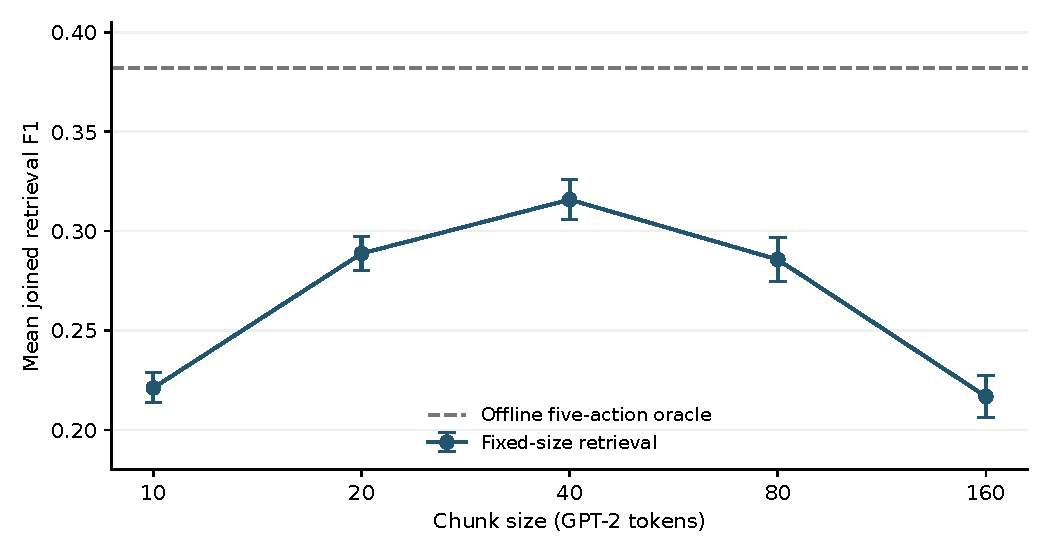
\includegraphics[width=\textwidth]{images/generated/fixed_granularity.pdf}
\caption{Fixed-size retrieval and the offline five-action oracle.
Error bars are 95\% paper-cluster bootstrap intervals for each fixed
method's mean, not intervals for all pairwise differences.}
\label{fig:fixed}
\end{figure}

The oracle reaches 0.3821, an absolute gain of 0.0662 over fixed 40.
Relative to the fixed-40 mean, this is approximately 21\% headroom.
The arithmetic describes the potential of selecting among the saved
actions; it does not predict how much of that potential a learner
can recover from observable features.

The exact retrieval-optimal size distribution includes every candidate:
138 questions prefer 10, 235 prefer 20, 282 prefer 40, 187 prefer 80,
and 82 prefer 160 under smaller-size tie-breaking. Thus fixed 40 is
the best aggregate setting without being the best action for most
individual questions. This is the strongest motivation for learning
an adaptive decision, and also a warning that the identity of the
best action can be difficult to predict.

The score diagnostics reveal a related tension. Mean query similarity
decreases from approximately 0.5490 at 10 tokens to 0.4271 at 160
tokens. Mean evidence similarity moves in the opposite direction,
from approximately 0.4538 to 0.5733. Joined retrieval F1 peaks between
the extremes. A router that simply maximises one similarity summary
therefore has no guarantee of optimising the primary metric.

\section{Early embedding and mixed-size experiments}
\subsection{Logistic regression versus the MLP}
The embedding router's logistic model achieves 0.2478 classification
accuracy and 0.2149 macro F1 against the legacy retrieval-derived
target. The MLP raises these to 0.2749 and 0.2187. Its macro-F1 gain
is only 0.0038, below the recorded 0.01 threshold for adopting the
more complex model.

The selected logistic router predicts counts
$(171,260,298,164,31)$ across the five sizes and reaches 0.2853
retrieval F1. It does not exceed fixed 40. The training-majority
legacy label is itself 40, and that constant reaches 0.3063
classification accuracy on validation, higher than either learned
classifier. Its macro F1 is much lower, 0.0938, because it predicts
only one class.

This comparison shows why no single classification summary tells
the full story. The learned model recognises more than one class,
but its errors cost enough retrieval quality to lose to a constant
size. The saved MLP result is a classification comparison only;
there is no full MLP retrieval score in the final baseline report.

\subsection{Raw and deduplicated mixtures}
Raw mixed-size retrieval reaches 0.2562 mean F1. Deduplication improves
it to 0.2618, but both remain below the selected embedding router
and the strongest fixed settings. The absolute deduplication gain
is approximately 0.0056.

\begin{table}[tbp]
\centering
\caption{Early adaptive baselines. The learned router uses the legacy
retrieval-derived label, not the later evidence-length target.}
\label{tab:early}
\begin{tabular}{@{}lrr@{}}
\toprule
Method & Mean retrieval F1 & Mean regret\\
\midrule
Question-embedding logistic router & 0.2853 & 0.0968\\
Mixed sizes, raw & 0.2562 & 0.1259\\
Mixed sizes, deduplicated & 0.2618 & 0.1203\\
\bottomrule
\end{tabular}
\end{table}

Of 4,620 raw mixed results, 2,708 are 10-token chunks and 1,148 are
20-token chunks. Together these account for more than 83\% of
returned chunks. Deduplication increases the 10-token count to
3,257, with 792 at 20 tokens. The procedure removes overlapping
spans after ranking; it does not recalibrate the ranking itself.
When a short candidate is ranked first, a larger containing passage
can subsequently be rejected.

The observed concentration on short chunks is consistent with the
cross-level query-score pattern. It is not sufficient to establish
that score scale is the only cause of mixed retrieval's lower F1.
Candidate counts, overlap, text boundaries, and the primary metric
also matter. The practical conclusion is narrower: raw pooling
and this overlap rule did not create a competitive adaptive baseline
in the evaluated setting.

\section{The question-only Qwen sequence}
% Generated by scripts/generate_results.py; do not hand-edit.
\begin{table}[htbp]
\centering\small
\caption{Question-only Qwen results on the evidence-length target.}
\label{tab:qwen_results}
\begin{tabular}{@{}llrrr@{}}
\toprule
Phase & Method & Accuracy & Macro F1 & Retrieval F1\\
\midrule
1 & Frozen Qwen & 0.0400 & 0.0490 & 0.2391\\
2 & Numeric SFT & 0.4318 & 0.1650 & 0.2266\\
2B-A & Uniform aliases & 0.3506 & 0.2092 & 0.2865\\
2B-B & Balanced aliases & 0.3701 & 0.1684 & 0.2496\\
2C & Base + class head & 0.3452 & 0.2176 & 0.2791\\
2D & Token-count prompt & 0.3690 & 0.2299 & 0.2767\\
2E & LR-grid winner & 0.3485 & 0.2278 & 0.2794\\
\bottomrule
\end{tabular}
\par\smallskip\begin{minipage}{\textwidth}\footnotesize Classification macro F1 and joined retrieval F1 measure different objectives.\end{minipage}
\end{table}


\subsection{Frozen prompting and numeric fine-tuning}
Phase 1 produces valid outputs for all 924 questions, but 767 predictions
are 10 tokens. Accuracy against evidence length is 0.0400 and macro
F1 is 0.0490. Its retrieval F1 is 0.2391. Valid formatting therefore
does not imply a useful decision.

Numeric fine-tuning changes the behaviour dramatically. The selected
Phase 2 checkpoint predicts 80 tokens 149 times and 160 tokens 775
times, never choosing the three smaller sizes. Accuracy rises to
0.4318 and macro F1 to 0.1650, while retrieval F1 falls to 0.2266.
Earlier checkpoints are even more concentrated on 160.

This is one of the clearest results in the thesis. The model has
become better at a proxy label while becoming worse at the evidence
retrieval task. Large evidence-length labels are common, particularly
in validation, but selecting five large chunks is a different action
from recovering that total evidence length. The result motivates a
change in supervision rather than an assumption that more training
alone will solve the mismatch.

For reference, a constant 80 prediction derived from the training
majority has validation accuracy 0.2511 and macro F1 0.0803. A
constant 160 prediction has validation accuracy 0.4545 and macro
F1 0.1250, but 160 is the validation majority rather than the
training majority. It is a descriptive comparison, not evidence
of a superior train-only baseline.

\subsection{Aliases and class balancing}
Uniform alias training in Phase 2B-A reaches macro F1 0.2092 and
retrieval F1 0.2865. It predicts 40 tokens 427 times, 80 tokens
189 times, and 160 tokens 308 times. This is a much less extreme
large-size distribution than numeric SFT, although the two smallest
classes remain unused.

Class-balanced alias training does not recover those missing classes.
Its selected second-epoch checkpoint predicts only 80 and 160, with
counts 434 and 490. Accuracy is slightly higher than in the uniform
variant, but macro F1 falls to 0.1684 and retrieval F1 to 0.2496.
Its top-two accuracy of 0.7056 exceeds the uniform variant's 0.6071,
which again does not make its top-one retrieval action better.

The controlled A/B experiment therefore gives no support for this
specific effective-number weighting scheme as an improvement. That
does not invalidate class weighting in general. The observed result
depends on a small, imbalanced dataset, the particular alias
formulation, a single recorded seed, and validation-selected
checkpoints.

\subsection{Classification head and explicit token counts}
The base-model classification head in Phase 2C reaches macro F1
0.2176 and retrieval F1 0.2791. It makes 20 predictions at size
20, but none at size 10. Its output distribution is less collapsed
than numeric SFT while still favouring medium and large sizes.

Changing only the instruction to explicit token counts in Phase 2D
raises accuracy from 0.3452 to 0.3690 and macro F1 from 0.2176
to 0.2299. Retrieval F1 moves in the opposite direction, from
0.2791 to 0.2767. Because neither prompt is truncated, the result
is not explained by the longer instruction removing question text.
The comparison supports an improvement in this classifier's label
prediction, not an improvement in the retrieval objective.

\subsection{Longer training and a learning-rate grid}
The Phase 2E winner, learning rate $5\times10^{-6}$ at epoch four,
achieves macro F1 0.2278 and retrieval F1 0.2794. It does not
exceed Phase 2D's macro F1, despite testing three learning rates
and fifteen epoch candidates. The best macro F1 in the other two
trials is approximately 0.2154 at $10^{-5}$ and 0.2252 at
$2\times10^{-5}$.

The small retrieval increase over Phase 2D is descriptive because
selection remains based on the repeatedly observed validation
classification metric. Only the selected global winner was evaluated
for final retrieval. The grid does not establish that longer
training is generally beneficial, nor that every checkpoint with
lower macro F1 would have lower retrieval F1.

\section{Similarity structure and feature fusion}
% Generated by scripts/generate_results.py; do not hand-edit.
\begin{table}[htbp]
\centering\small
\caption{Global similarity-tree and fusion results on the evidence-length target.}
\label{tab:tree_results}
\begin{tabular}{@{}llrrr@{}}
\toprule
Phase & Method & Accuracy & Macro F1 & Retrieval F1\\
\midrule
3A & Linear tree router & 0.3030 & 0.1928 & 0.2677\\
3B & XGBoost tree router & 0.3290 & 0.2247 & 0.2717\\
3C & Original fusion & 0.3193 & 0.2307 & 0.2872\\
3C-OOF & Corrected fusion & 0.3225 & 0.2100 & 0.2783\\
\bottomrule
\end{tabular}
\par\smallskip\begin{minipage}{\textwidth}\footnotesize Classification macro F1 and joined retrieval F1 measure different objectives. Original fusion has in-sample base-feature contamination in its training-fold evaluation.\end{minipage}
\end{table}


\subsection{From linear score features to boosted trees}
The Phase 3A full-tree linear model reaches validation macro F1
0.1928 and retrieval F1 0.2677. Its level-only counterpart has
macro F1 0.1892. The difference is small, and the selected
level-only model has slightly higher training OOF macro F1 than
the selected tree model, approximately 0.2253 versus 0.2222.
There is no consistent large hierarchy gain in this linear setup.

The heuristic diagnostics are also limited. Maximum similarity and
top-five mean similarity have validation macro F1 of 0.0600 and
0.0573. The training-tuned penalised score reaches 0.1434, while
the leaf-breadth rule reaches 0.1242. The latter's accuracy is
0.3755, illustrating again how a comparatively favourable accuracy
can coexist with weak class-balanced performance.

XGBoost improves the primary full-tree result in Phase 3B to
macro F1 0.2247 and retrieval F1 0.2717. The retrieval increase
over the linear tree model is about 0.0040. The level-only
XGBoost model has validation macro F1 0.1822. Nonlinear use of
the full representation is more promising than the particular
linear model, but the retrieval outcome is still below fixed
20, fixed 40, and the strongest question-only alias variant.

Score features therefore contain some usable information without
making the evidence-length proxy an effective retrieval objective.
The results should not be read as proving that a literal hierarchy
is intrinsically superior to all flat representations; the models,
feature definitions, and small hyperparameter grids define the
scope of that comparison.

\subsection{Original fusion and its corrected rerun}
Original Phase 3C fusion reaches macro F1 0.2307 and retrieval F1
0.2872. These are improvements over the primary Phase 3B result.
However, the training-fold fusion estimate uses in-sample Qwen
features, as explained in Chapter~\ref{ch:method}.

The exploratory hidden-state fusion has validation accuracy 0.3203
and macro F1 0.2298, close to the logits variant. Its training-fold
macro F1 is 0.3544, below the logits variant's 0.3838, so the
compact logits representation is retained. The hidden-state variant
does not have the primary final retrieval evaluation.

The corrected OOF experiment reduces the apparent training-fold
macro F1 from approximately 0.3838 to 0.2317, and accuracy from
0.4717 to 0.3042. The external validation result is macro F1
0.2100 and retrieval F1 0.2783, below the original fusion by
approximately 0.0089 retrieval F1.

It would be misleading to describe this only as a failed attempt to
improve a score. The corrected training interface answers a more
credible question. Its lower result indicates that the earlier
optimism cannot be carried forward unchanged. The rerun preserves
the useful idea of combining signals while removing an identifiable
source of training contamination.

\begin{figure}[tbp]
\centering
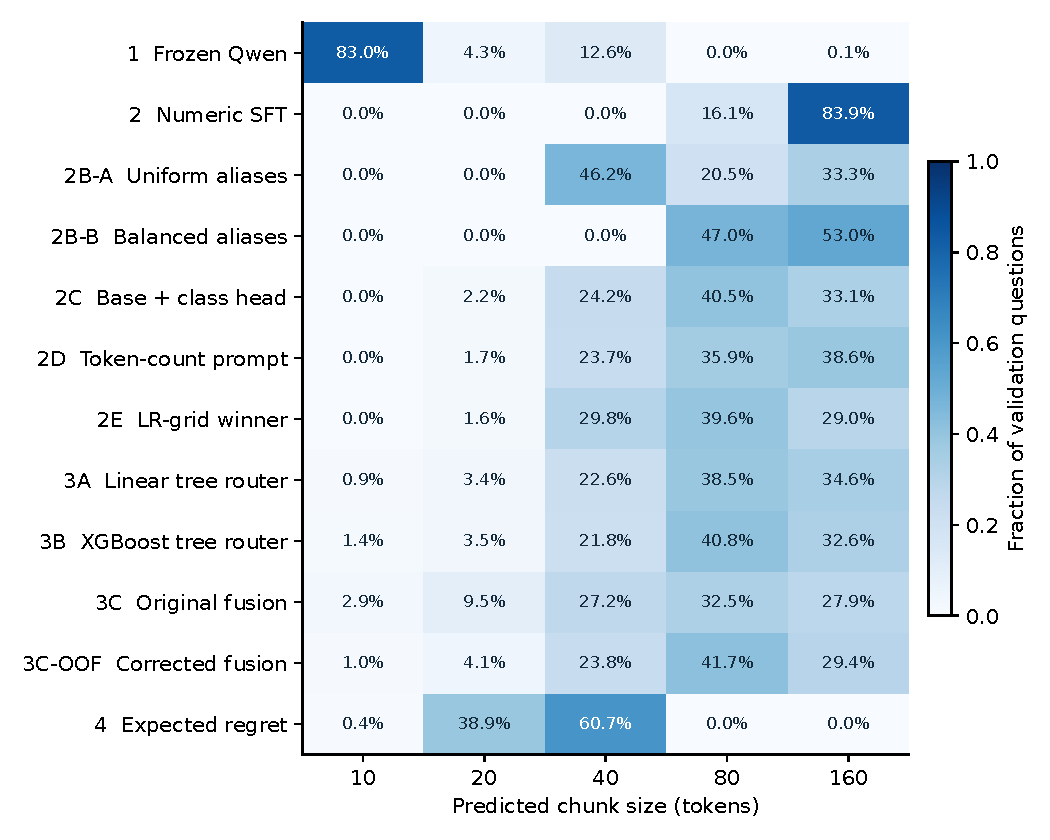
\includegraphics[width=\textwidth]{images/generated/prediction_heatmap.pdf}
\caption{Predicted granularity distributions across the main
question-level phases. Rows sum to 100\%. Phase 4 optimises retrieval
regret; the preceding rows use evidence-length classification.}
\label{fig:predictions}
\end{figure}

Figure~\ref{fig:predictions} shows why aggregate label metrics need
the accompanying prediction distributions. Most evidence-length
classifiers assign many questions to 80 or 160. The expected-regret
router discussed next behaves differently even though it uses
the same families of observable features as corrected fusion.

\section{Expected regret: the strongest learned global router}
Phase 4 reaches mean retrieval F1 0.3075 and median F1 0.3008.
Its mean regret is 0.0746. It chooses 10 tokens for four questions,
20 for 359, and 40 for 561; it never selects 80 or 160 on validation.
Compared with the preceding evidence-length models, the decision
distribution shifts strongly towards the sizes that perform well
under joined retrieval F1.

% Generated by scripts/generate_results.py; do not hand-edit.
\begin{table}[htbp]
\centering\small
\caption{Expected-regret router (Phase 4) minus each comparator.}
\label{tab:pairedregret}
\begin{tabular}{@{}lrr@{}}
\toprule
Comparator & Mean F1 difference & 95\% interval\\
\midrule
2D & +0.03079 & [+0.02174, +0.04003]\\
3B & +0.03579 & [+0.02663, +0.04483]\\
Original 3C & +0.02030 & [+0.01162, +0.02877]\\
3C-OOF & +0.02920 & [+0.01987, +0.03864]\\
Fixed 40 & -0.00835 & [-0.01266, -0.00416]\\
\bottomrule
\end{tabular}
\par\smallskip\begin{minipage}{\textwidth}\footnotesize Paired paper-cluster bootstrap with 10,000 replicates and seed 42. Positive values favour Phase 4.\end{minipage}
\end{table}


The paired comparisons in Table~\ref{tab:pairedregret} favour Phase 4
over Phase 2D, Phase 3B, original fusion, and corrected fusion.
The respective mean gains are 0.0308, 0.0358, 0.0203, and 0.0292.
Their paper-cluster intervals exclude zero in the observed development
sample. These results support the practical value of aligning the
training target with retrieval utility.

\begin{figure}[tbp]
\centering
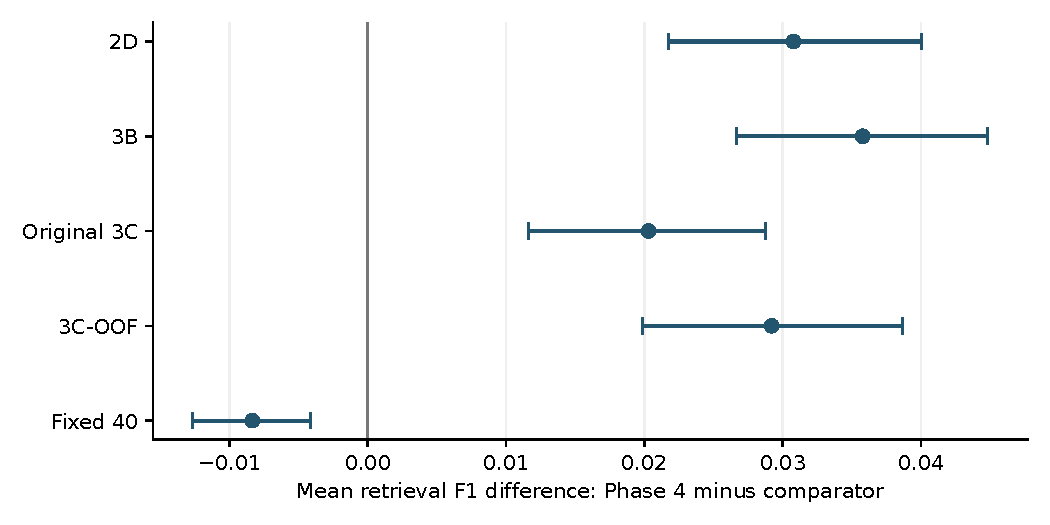
\includegraphics[width=\textwidth]{images/generated/regret_differences.pdf}
\caption{Paired mean retrieval-F1 differences for Phase 4. Intervals
are obtained by resampling papers, not by retraining the models.}
\label{fig:regret}
\end{figure}

The main baseline remains stronger. Phase 4 minus fixed 40 is
$-0.00835$, with interval $[-0.01266,-0.00416]$. Consequently,
the strongest learned question-level router in the repository does
not establish an advantage over fixed 40. It narrows the gap left
by the earlier learned methods without closing it.

The fraction of questions with zero regret is 280/924, or 0.3030.
This allows any equally optimal action. Accuracy against an exact
smaller-tie label is slightly different, 0.3019. Neither should
be substituted for the other. Against the evidence-length labels,
Phase 4 has accuracy only 0.1418 and macro F1 approximately 0.1060.
That low proxy score is entirely compatible with its stronger
retrieval outcome.

The absence of large-size predictions is also a limitation. The
oracle still prefers 80 or 160 for many questions. The model
appears to learn a useful conservative preference without reliably
identifying those exceptions. A good average action is not the
same as a successful instance-level explanation of evidence need.

\section{Three concrete routing cases}
The following cases are drawn directly from the frozen validation
records, with the original question wording retained. The first is
the largest Phase 4 gain over fixed 40, the second the largest loss,
and the third illustrates a near tie. They are deliberately selected
diagnostics, not a random sample or an estimate of how often each
pattern occurs.

% Generated, deliberately selected diagnostic cases; not a random sample.
\par\medskip\noindent\begin{minipage}{\textwidth}
\textbf{Case 1: Did they collect their own datasets?}\par\smallskip
Paper 1608.01884. Phase 4 selects 10 tokens. The F1 difference from fixed 40 is $+0.277200$.
\begin{center}\small\begin{tabular}{@{}lrrrrr@{}}\toprule
Size & 10 & 20 & 40 & 80 & 160\\\midrule
Retrieval F1 & 0.5432 & 0.3103 & 0.2660 & 0.1552 & 0.1291\\
\bottomrule\end{tabular}\end{center}
\end{minipage}\par\medskip

\par\medskip\noindent\begin{minipage}{\textwidth}
\textbf{Case 2: Did they used dataset from another domain for evaluation?}\par\smallskip
Paper 1909.03582. Phase 4 selects 20 tokens. The F1 difference from fixed 40 is $-0.322390$.
\begin{center}\small\begin{tabular}{@{}lrrrrr@{}}\toprule
Size & 10 & 20 & 40 & 80 & 160\\\midrule
Retrieval F1 & 0.2357 & 0.3032 & 0.6256 & 0.8213 & 0.5610\\
\bottomrule\end{tabular}\end{center}
\end{minipage}\par\medskip

\par\medskip\noindent\begin{minipage}{\textwidth}
\textbf{Case 3: What experiments are conducted?}\par\smallskip
Paper 1909.06200. Phase 4 selects 20 tokens. The F1 difference from fixed 40 is $+0.003092$.
\begin{center}\small\begin{tabular}{@{}lrrrrr@{}}\toprule
Size & 10 & 20 & 40 & 80 & 160\\\midrule
Retrieval F1 & 0.1750 & 0.3636 & 0.3605 & 0.3097 & 0.1997\\
\bottomrule\end{tabular}\end{center}
\end{minipage}\par\medskip


In the first case, a rare 10-token decision is useful: its F1 is
0.5432, above all four larger alternatives. This demonstrates that
the router is not simply a disguised constant-40 method. In the
second case, the 20-token decision misses a substantial opportunity:
80-token retrieval reaches 0.8213 while the chosen action reaches
0.3032. The question's short wording alone does not justify a
short evidence window.

The third case explains why a cost-sensitive target can be more
informative than a hard class. Choosing 40 instead of the optimal
20 would lose only about 0.0031 F1. A classification metric marks
that decision wrong, just as it marks a much more damaging choice
wrong. Regret preserves the difference in severity.

These examples describe observed utility patterns. They do not
show that any model generated a correct answer, and they do not
establish the semantic sufficiency of the retrieved chunks without
separate evidence inspection.

\section{Local tree-level retrieval}
% Generated by scripts/generate_results.py; do not hand-edit.
\begin{table}[htbp]
\centering\small
\caption{Matched local retrieval: five ranked trees, one chunk per tree.}
\label{tab:localresults}
\begin{tabular}{@{}lrrrr@{}}
\toprule
Method & Precision & Recall & F1 & Tokens\\
\midrule
Same-tree fixed 10 & 0.3829 & 0.1932 & 0.2195 & 53.8\\
Same-tree fixed 20 & 0.3440 & 0.3237 & 0.2820 & 103.6\\
Same-tree fixed 40 & 0.2846 & 0.4862 & 0.3075 & 202.7\\
Same-tree fixed 80 & 0.2103 & 0.6469 & 0.2791 & 400.5\\
Same-tree fixed 160 & 0.1385 & 0.7833 & 0.2135 & 792.5\\
Phase 5A local & 0.2754 & 0.5114 & 0.3053 & 232.8\\
Phase 5B-v2 & 0.2739 & 0.5120 & 0.3045 & 234.8\\
\bottomrule
\end{tabular}
\par\smallskip\begin{minipage}{\textwidth}\footnotesize Each score is a mean over 924 questions. Tokens are measured in the saved retrieval output, not inferred from nominal chunk size.\end{minipage}
\end{table}


Phase 5A returns one chunk from each of five selected trees and
achieves mean precision 0.2754, recall 0.5114, and F1 0.3053.
The matched same-tree fixed-40 method reaches precision 0.2846,
recall 0.4862, and F1 0.3075. Local adaptation gains some recall
but loses enough precision that its F1 is slightly lower.

The paired difference is $-0.00220$, with a 95\% paper-cluster
interval of $[-0.00580,0.00145]$. The observed difference does
not demonstrate a local-routing advantage. The interval also does
not establish that the two methods are equivalent; an equivalence
claim would need an explicit margin and an appropriate test.

Phase 5A makes 4,620 local size predictions, with counts
$(246,529,2823,965,57)$. Forty tokens dominates, which is consistent
with its role as a strong local default. The mean retrieved token
count is 232.8, compared with 202.7 for the same-tree fixed-40
method. Equal chunk counts therefore still leave a difference
in text budget.

The secondary gold-overlap classification diagnostic has accuracy
0.2850 and macro F1 0.2144. It helps assess the local target but
does not evaluate how well the method selected the five trees:
those diagnostic examples are constructed using gold overlap,
whereas inference ranks all available trees without gold.

Returning all chunks at the predicted level changes the outcome
substantially. Mean recall rises to 0.7826, but precision falls to
0.1382 and F1 to 0.2131. The method now returns an average of
22.44 chunks and 809.5 tokens. This exploratory result demonstrates
the cost of indiscriminate coverage within selected regions, not
an improvement under the primary top-five budget.

Global fixed 40 and same-tree fixed 40 must remain separate.
Their F1 values are 0.3159 and 0.3075, respectively. Requiring
one chunk per root imposes spatial diversity and can exclude
multiple useful chunks from one region. The matched local baseline
is therefore essential for isolating the router's contribution.

\section{The final Qwen context-feature experiment}
\subsection{An invalid-output failure that was not hidden}
The first Phase 5B version produces 175 invalid outputs among
2,101 eligible training questions and 56 among 924 validation
questions. There are 231 invalid outputs in total. Among valid
training categories, the counts are 54 short, 1,867 medium, and
five long; validation has 31 short, 836 medium, and one long.

Some outputs answer the underlying question rather than estimate
context need. A default category would hide that interface failure.
The pipeline instead stops before downstream classifier training.
This version has no final retrieval score and is not treated as
a completed ablation with poor performance.

\subsection{Valid constrained outputs, little additional information}
The training-only wording repair succeeds on 173 of the 175
previous failures under its probe. Two failures remain, motivating
the constrained first-token decision. The final Phase 5B-v2
feature has no invalid outputs, but its distribution is highly
concentrated: training has 24 short, 2,076 medium, and one long;
validation has 12 short, 912 medium, and no long.

Thus 98.70\% of validation questions receive the same category.
The feature is correctly formatted but has very little variation.
The resulting local router reaches retrieval F1 0.3045, compared
with 0.3053 for Phase 5A. The difference is $-0.00073$, with
interval $[-0.00236,0.00088]$. Against same-tree fixed 40, the
difference is $-0.00293$, with interval $[-0.00646,0.00069]$.
Neither comparison demonstrates an improvement.

The local prediction distribution changes slightly to
$(247,506,2804,1008,55)$, and secondary local classification
accuracy and macro F1 are approximately 0.2811 and 0.2123.
The added feature therefore changes the fitted decisions, but
not in a way supported as beneficial by the primary outcome.
Output validity and feature usefulness are separate requirements.

\section{Engineering and computational observations}
The repository records substantial work that does not correspond
to a new row of retrieval F1: ingestion retries, smoke tests,
tiny-overfit checks, accumulation-tail preflights, checkpoint
recovery, score audits, feature extraction resumption, and
pre-evaluation hash locks. Their role is to establish that the
reported row means what it claims to mean.

The corrected fusion procedure illustrates the additional training
cost of methodological care. The recorded total is about 7,712
seconds, or two hours and eight minutes, including five fold
fits, a full-data refit, feature extraction, meta-model fitting,
and retrieval evaluation. The five fold fits account for about
5,888 seconds and the refit for about 1,434 seconds. Maximum
recorded allocated GPU memory is approximately 9.03 GB, with
9.60 GB reserved.

These figures describe that recorded execution, not a general
latency benchmark. Earlier zero-shot generation, GPU fine-tuning,
CPU tree fitting, cached feature use, and live retrieval have
different hardware and timing boundaries. Comparing their wall
times as though they were interchangeable online requests would
be misleading.

At prediction time, a question-only router can choose a size
before retrieval. A similarity-tree router needs similarities
across the paper and all levels before deciding. Even if many
values are cached, that extra information has an acquisition
cost. The current study measures retrieval quality more completely
than end-to-end deployment efficiency. A future system should
report both the cost of feature construction and the cost of
the final returned context.

\section{Threats to validity}
\subsection{Repeated validation and limited random seeds}
The most important limitation is repeated validation use.
Checkpoint selection, prompts, representations, and subsequent
research directions were informed by this split over time.
Training-only decisions in later phases improve local experimental
discipline but do not erase that history. The thesis therefore
does not present the final numbers as untouched test performance.

Most main training results use one recorded seed. Bootstrap
intervals resample evaluation papers while holding fitted models
fixed; they do not quantify the variation across independent
training runs. The many development comparisons also create a
multiple-comparison context. Intervals are reported for specified
pairs without claiming a family-wide corrected discovery.

\subsection{Metric and budget validity}
Joined token F1 measures lexical agreement with annotated
evidence. It can penalise helpful explanatory context and reward
matching tokens that occur outside the annotated source span.
It does not evaluate factual correctness, entailment, citation
accuracy, or answer generation. Its values should not be
presented as a full RAG quality score.

The fixed-size comparisons hold the chunk count constant while
allowing the total text budget to vary. Local routing holds
the number of selected trees and returned chunks constant, but
still changes total length. The results identify useful settings
under those protocols; a constant-token-budget experiment could
lead to a different ranking.

\subsection{Data and representation validity}
The study uses scientific NLP papers, a single fixed embedding
model, a small discrete size set, and paper-restricted retrieval.
Sentence-aware chunks, contextual chunk embeddings, other
domains, corpus-level negatives, and different annotation
practices may change the behaviour.

The local target further depends on evidence that can be mapped
to text offsets. Partial mappings and excluded table/figure
evidence create a selection effect. The primary validation
retrieval includes all frozen questions, but the local classifier
learns from a narrower subset of evidence types.

\subsection{Causal interpretation}
The sequence contains both controlled ablations and broader
redesigns. A prompt-only change supports a narrower conclusion
than a change of model family, feature source, and target.
The thesis avoids treating every later phase as proof that
one named component caused a gain. The strongest defensible
interpretation is comparative: under the preserved configurations,
utility-aware learning improved the learned global decision,
while neither global nor local adaptation surpassed its
strong fixed-size reference.

\section{Synthesis}
Three lessons recur across the experimental history. First,
the target is decisive. Evidence length is interpretable but
does not directly describe the utility of five retrieved chunks.
Second, more information is useful only when it is both validly
constructed and informative: corrected OOF fusion reduces
optimism, while constrained Qwen outputs fix formatting without
creating category diversity. Third, a fixed baseline deserves
to remain in every comparison. Here it prevents a progression
of increasingly complex methods from being mistaken for a
progression of consistently better retrieval systems.
